\newpage
\section{Usando toxtren}
En esta sección vamos a hacer un recorrido por el toolbox toxtren, de modo que el usuario podrá ver fácilmente cómo trabajar con el mismo. Haremos un repaso sobre los métodos esenciales y más importantes para el manejo de trenzas y trenzas cerradas. \\
 

\subsection{Clase trenza.}

\begin{center}
	\textbf{Constructor.}
\end{center}
En primer lugar vamos a ver el constructor para dicha clase. Podemos crear una trenza indicando los cruces de la trenza y el número de cadenas de la misma. Por ejemplo, creamos la trenza $\sigma1\sigma2^{-1}\sigma1^{-1}$ con 5 cadenas del siguiente modo:
	\lstset{language=Matlab, breaklines=true, basicstyle=\ttfamily\small}
\begin{lstlisting}
>> a=trenza([1 -2 -1],5)
\end{lstlisting}
	\lstset{emph=[1]{trenza,trenza_cerrada},emphstyle=[1]\color{blue}}
\begin{lstlisting}
	a = trenza with properties:
	    indices_trenza: [1 -2 -1]
	    n_cadenas: 5
\end{lstlisting}

Si no indicamos el número de cadenas de la trenza, se establecerá al número mínimo de cadenas que tendrá que tener. 
   \lstset{emph=[1]{trenza,trenza_cerrada},emphstyle=[1]\color{black}}
\begin{lstlisting}
>> a=trenza([1 -2 -1])
\end{lstlisting}
\lstset{emph=[1]{trenza,trenza_cerrada},emphstyle=[1]\color{blue}}
\begin{lstlisting}
	a = trenza with properties:
	    indices_trenza: [1 -2 -1]
	    n_cadenas: 3
\end{lstlisting}

Además para ambos casos podemos indicar la trenza mediante una cadena tal y cómo hemos comentado al inicio del capítulo:

\lstset{emph=[1]{trenza,trenza_cerrada},emphstyle=[1]\color{black}}
\begin{lstlisting}
>> b=trenza('+s3-s2',7)
\end{lstlisting}
\lstset{emph=[1]{trenza,trenza_cerrada},emphstyle=[1]\color{blue}}
\begin{lstlisting}
b = trenza with properties:
indices_trenza: [3 -2]
n_cadenas: 7
\end{lstlisting}

Del mismo modo que antes, si no indicamos el número de cadenas de la trenza se establecerá como el número mínimo que ha de tener. 
\lstset{emph=[1]{trenza,trenza_cerrada},emphstyle=[1]\color{black}}
\begin{lstlisting}
>> b=trenza('+s3-s2')
\end{lstlisting}
\lstset{emph=[1]{trenza,trenza_cerrada},emphstyle=[1]\color{blue}}
\begin{lstlisting}
	b = trenza with properties:
	    indices_trenza: [3 -2]
	    n_cadenas: 4
\end{lstlisting}



\newpage
\begin{center}
	\textbf{Operaciones básicas.}
\end{center}
Obtenemos la trenza potencia de una trenza.
\begin{lstlisting}
>> pote(a,3)
	ans = trenza with properties:
	      indices_trenza: [1 -2 -1 1 -2 -1 1 -2 -1] 
	      n_cadenas: 3
\end{lstlisting}


Podemos obtener la trenza producto de un par de trenzas.
\begin{lstlisting}
>> c=producto(a,b)
	c = trenza with properties:
	    indices_trenza: [1 -2 -1 3 -2]
	    n_cadenas: 4
\end{lstlisting}

Obtenemos la trenza inversa de una trenza haciendo uso de la función inver:
\begin{lstlisting}
>> c.inver
	ans = trenza with properties:
	      indices_trenza: [2 -3 1 2 -1]
	      n_cadenas: 4
\end{lstlisting}

Podemos obtener el número de cruces de una trenza del siguiente modo:
\begin{lstlisting}
>> c.length
	ans =5
\end{lstlisting}

\begin{center}
	\textbf{Get/Set.}
\end{center}
Podemos obtener los cruces y el número de cadenas de una trenza con los siguientes get. 
\begin{lstlisting}
>> a.get_indices
ans = 1    -2    -1
\end{lstlisting}

\begin{lstlisting}
>> a.get_n
ans = 3
\end{lstlisting}

Cambiamos el número de cadenas de una trenza del siguiente modo:
\begin{lstlisting}
>> set_n(a,6)
>> a
a = trenza with properties:
indices_trenza: [1 -2 -1]
n_cadenas: 6
\end{lstlisting}

Finalmente cambiamos los cruces de la trenza:
\begin{lstlisting}
>> set_indices(a,[4 -3])
>> a
a = trenza with properties:
indices_trenza: [4 -3]
n_cadenas: 5
\end{lstlisting}
Si no indicamos un tercer parámetro que representa el número de cadenas de la trenza modificada, se establecerá al número de cadenas por defecto. 

\newpage
\begin{center}
	\textbf{Invariantes básicos.}
\end{center}
Para ver los invariantes básicos vamos a trabajar con la trenza que hemos creado anteriormente:
\begin{lstlisting}
>> a
	a = trenza with properties:
	    indices_trenza: [4 -3]
	    n_cadenas: 5
\end{lstlisting}

Obtenemos el invariante exponente mediante el método exp:
\begin{lstlisting}
>> a.exp
	ans = 0
\end{lstlisting}

Obtenemos la permutación de la trenza:
\begin{lstlisting}
>> a.perm	
	ans = 1     2     4     5     3
\end{lstlisting}

A partir de esta permutación podemos ver si la trenza es pura. Al obtener respuesta negativa, sabemos que la trenza no es pura. 
\begin{lstlisting}
>> a.pura	
	ans = 0
\end{lstlisting}

\begin{center}
	\textbf{Otros métodos destacados.}
\end{center}
Podemos ver la representación 3D de una trenza del siguiente modo:
\begin{lstlisting}
>> a.representar_trenza
\end{lstlisting}
\begin{figure}[h!]
	\centering
	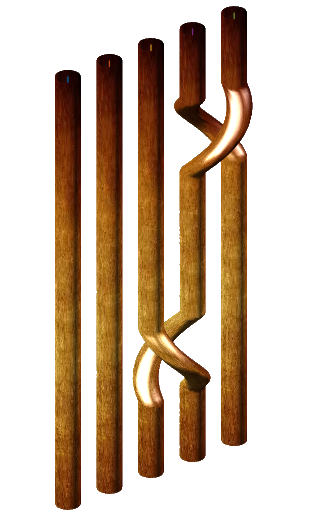
\includegraphics[width=5cm]{img/infor1.png}
	\caption{Representación trenza Matlab.}
	\label{inf1} 
\end{figure}

\newpage
Para aplicar el algoritmo de Dehornoy sobre una trenza y ver su representación, vamos a crear una nueva trenza más compleja y haremos uso del siguiente comando:

\lstset{emph=[1]{trenza,trenza_cerrada},emphstyle=[1]\color{black}}
\begin{lstlisting}
>> a=trenza([1 -2 2 2 -1])
\end{lstlisting}
\lstset{emph=[1]{trenza,trenza_cerrada},emphstyle=[1]\color{blue}}
\begin{lstlisting}
	a = trenza with properties:
	    indices_trenza: [1 -2 2 2 -1]
	    n_cadenas: 3
>> [e_trivial,final]=a.dehornoy
	e_trivial = 0
	final = -2     1     2
\end{lstlisting}
Podemos ver el principio y final del proceso en la figura \ref{inf2}
\begin{figure}[h!]
	\centering
	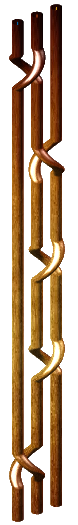
\includegraphics[width=1.2cm]{img/infor2.png}
	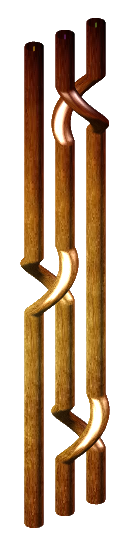
\includegraphics[width=2cm]{img/infor3.png}
	\caption{Transformación Dehornoy Matlab.}
	\label{inf2} 
\end{figure}

Creamos una trenza a partir de los cruces que hemos obtenido al aplicar el algoritmo de Dehornoy a la trenza a:
\lstset{emph=[1]{trenza,trenza_cerrada},emphstyle=[1]\color{black}}
\begin{lstlisting}
>> f=trenza(final)
\end{lstlisting}
\lstset{emph=[1]{trenza,trenza_cerrada},emphstyle=[1]\color{blue}}
\begin{lstlisting}
	f = trenza with properties:
	    indices_trenza: [-2 1 2]
	    n_cadenas: 3
\end{lstlisting}

Obviamente al aplicar el algoritmo de equivalencia entre las trenzas a y f tendremos que obtener respuesta afirmativa:
\begin{lstlisting}
>> equivalentes(a,f)
	ans = 1
\end{lstlisting}

Finalmente podemos comprobar si una trenza dada es o no trivial. En este caso la trenza a no es equivalente a la trenza trivial. 
\begin{lstlisting}
>> a.es_trivial
	ans = 0
\end{lstlisting}

\subsection{Clase trenza\_cerrada.}

\begin{center}
	\textbf{Constructor.}
\end{center}
Podemos obtener una trenza cerrada a partir de un vector que contiene los cruces o bien indicando la cadena de cruces, al igual que hacíamos con las trenzas. Del mismo modo, podemos indicar el número de cadenas que tendrá la cadena o establecerlo al número mínimo por defecto. Vamos a ver un ejemplo entre estas cuatro opciones posibles:
\lstset{emph=[1]{trenza,trenza_cerrada},emphstyle=[1]\color{black}}
\begin{lstlisting}
>> m=trenza_cerrada([3 -1 2],5)
\end{lstlisting}
\lstset{emph=[1]{trenza,trenza_cerrada},emphstyle=[1]\color{blue}}
\begin{lstlisting}
	m = trenza_cerrada with properties:
	    n_enlaces: 1
	    indices_trenza: [3 -1 2]
	    n_cadenas: 5
\end{lstlisting}

Además, podemos crear una trenza cerrada a partir de una trenza dada. Vamos a crear la trenza cerrada a\_c a partir de la trenza a que creamos anteriormente:
\begin{lstlisting}
>> a
	a = trenza with properties:
	    indices_trenza: [1 -2 2 2 -1]
	    n_cadenas: 3
\end{lstlisting}
\lstset{emph=[1]{trenza,trenza_cerrada},emphstyle=[1]\color{black}}
\begin{lstlisting}
>> a_c=trenza_cerrada(a)
\end{lstlisting}
\lstset{emph=[1]{trenza,trenza_cerrada},emphstyle=[1]\color{blue}}
\begin{lstlisting}	    
	a_c = trenza_cerrada with properties:	    
	    n_enlaces: 2
	    indices_trenza: [1 -2 2 2 -1]
	    n_cadenas: 3
\end{lstlisting}

Los métodos get/set y los relativos a operaciones e invariantes básicos se llaman del mismo modo que hemos visto para trenzas. Por este motivo, para trenzas cerradas vamos a mostrar solamente la sección de otros métodos destacados. 

\bigskip
\begin{center}
	\textbf{Otros métodos destacados. }
\end{center}
Podemos obtener la notación de Dowker de una trenza cerrada de un sólo enlace con el siguiente método:
\begin{lstlisting}
>> m.Dowker
	ans = 6    -4     2
>> a_c.Dowker
	Se trata de un enlace.
\end{lstlisting}

Obtenemos el polinomio de Alexander de una trenza cerrada:
\lstset{emph=[1]{trenza,trenza_cerrada},emphstyle=[1]\color{black}}
\begin{lstlisting}
>> aux=trenza_cerrada([ 1 2 3])
\end{lstlisting}
\lstset{emph=[1]{trenza,trenza_cerrada},emphstyle=[1]\color{blue}}
\begin{lstlisting}
	aux = trenza_cerrada with properties:
	    n_enlaces: 1
	    indices_trenza: [1 2 3]
	    n_cadenas: 4
>> aux.Alexander
	ans = -1
\end{lstlisting}

Podemos ver la representación 3D de una trenza cerrada haciendo uso de representar\_trenza. Aunque para el caso de trenzas no lo comentamos, a dicho método le podemos para el número de cortes que tendrán las cadenas y el radio de las mismas.\\
Por ejemplo, visualizamos la trenza cerrada m con un radio de 0.4 y 30 cortes por cadena del siguiente modo:

\begin{lstlisting}
>> representar_trenza(m,30,0.4)
\end{lstlisting}
\begin{figure}[h!]
	\centering
	
\includegraphics[width=4.3cm]{img/infor4.png}
	\caption{Representación trenza cerrada Matlab.}
	\label{inf3} 
\end{figure}

Podemos ver si dos trenzas cerradas son equivalentes. Además, podemos pedir mensajes explicativos que nos muestren porqué las trenzas cerradas son o no equivalentes. Este detalle también es posible realizarlo para trenzas, simplemente tenemos que indicarlo con un nuevo parámetro.  
\begin{lstlisting}
>> equivalentes(a_c,m,1)
	Las trenzas cerradas no son equivalentes porque tienen distinto numero de enlaces.
	ans = 0
\end{lstlisting}

Finalmente podemos ver si una trenza cerrada es equivalente a la trivial, y mostrar o no mensajes de salida explicativos.
\lstset{emph=[1]{trenza,trenza_cerrada},emphstyle=[1]\color{black}}
\begin{lstlisting}
>> es_trivial(m,true)
	La trenza dada no es equivalente a la trenza trivial. Su exponente no es nulo.
	Pero es posible que la trenza cerrada si sea equivalente a la trivial.
	Comparando los polinomios de Alexander obtenemos que...
	La trenza cerrada no es equivalente a la trivial.
	ans = 0
\end{lstlisting}
